\section{Equilibrio idrostatico}\label{sec:equilibrio-idrostatico}
L'equazione dell'\emph{equilibrio idrostatico} esprime la condizione per cui la pressione interna del gas che compone la stella è in equilibrio con la forza di gravità data dalla massa della stella stessa. Si può riassumere nella seguente maniera:
\begin{equation}\label{eq:equilibrio-idrostatico}
    \dfrac{\ud P(r)}{\ud r} = -\dfrac{G M(r)}{r^2} \rho(r)
\end{equation}

\begin{figure}
\centering
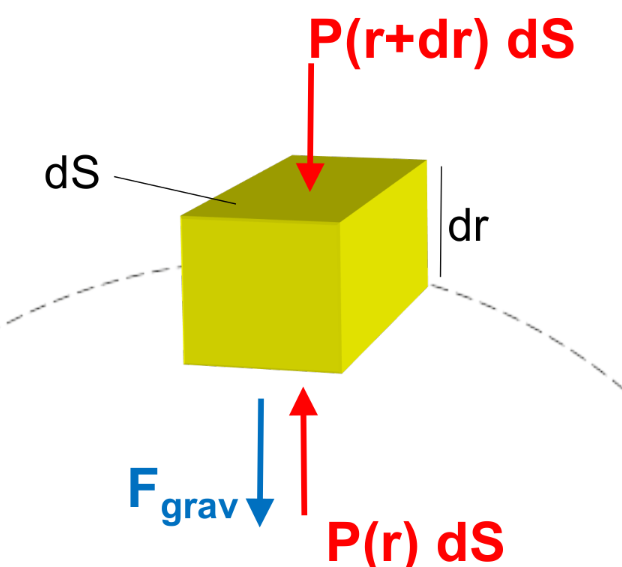
\includegraphics[width=0.3\textwidth]{immagini/equilibrio-idrostatico.png}
\caption{Volumetto infinitesimo a distanza $r$ dal centro della stella. Sulla faccia superiore agiste la pressione che spinge verso il centro. Sulla faccia inferiore agiscono la pressione, verso l'esterno, e la forza di gravità, verso il centro.}
\label{fig:equilibrio-idrostatico}
\end{figure}

Per ricavare tale equazione immaginiamo di dividere la stella in gusci sferici concentrici a temperatura e densità costanti; ognuno di questi è caratterizzato da un valore di densità e di temperatura decrescenti all'aumentare dalla distanza dal centro. Consideriamo un volume infinitesimo di stella a una distanza $r$ dal centro; come mostrato in figura~\ref{fig:equilibrio-idrostatico}, sulla faccia esterna del volumetto agisce una forza di pressione verso l'interno, mentre sulla faccia interna agisce una forza di pressione verso l'esterno e la forza gravitazionale, verso l'interno. Scriviamo quindi l'espressione per la forza di pressione $F_p$ e la forza di gravità $F_g$ e le poniamo uguali per imporre la condizione di equilibrio. Si tenga conto che l'asse radiale è rivolto verso il centro, sicché le forse che agiscono verso l'esterno avranno segno negativo.
\[
    F_p = P(r+\ud r) \ud S - P(r) \ud S = \frac{\ud P(r)}{\ud r} \ud r \ud S
\]
\[
    F_g = \frac{GM(r)}{r^2} \rho(r) \ud r \ud S
\]
dove $M(r)$ rappresenta la massa all'interno del raggio $r$, il termine $GM(r) / r^2$ rappresenta l'accelerazione locale di gravità e il termine $\rho(r) \ud r \ud S$ rappresenta la massa all'interno del volumetto. Imponendo l'equilibrio si trova:
\[
    F_p + F_g = 0 \iff \frac{\ud P(r)}{\ud r} \ud r \ud S+ \frac{GM(r)}{r^2} \rho(r) \ud r \ud S = 0
\]
da cui segue immediatamente l'eq.~\eqref{eq:equilibrio-idrostatico}. Quindi, in ogni guscio sferico della stella a fissata distanza $r$ dal centro, la gravità è bilanciata dalla pressione interna del gas. In particolare, la gravità \emph{non} è bilanciata dalla pressione, più precisamente essa è bilanciata dal \emph{gradiente di pressione}, ovvero dalla variazione di $P$ col raggio. La pressione deve decrescere all'aumentare del raggio, sicché la pressione nel centro della stella è maggiore della pressione vicino alla sua superficie. 

Quando $F_g$ e $F_p$ \emph{non} sono bilanciate, la stella si contrae per $F_g > F_p$ o espande per $F_g < F_p$ in un \emph{tempo caratteristico} pari a:
\[
    T_d = \sqrt{\frac{2r}{g}} = \sqrt{\frac{2r^3}{GM}}
\]

Ci potremmo chiedere quanto ci vorrebbe per una stella come il Sole a collassare se la pressione scomparisse improvvisamente: utilizzando l'equazione qui sopra otterremmo un tempo di circa 38 minuti.